\documentclass{article}
\usepackage[utf8]{inputenc}
\usepackage{graphicx}
\usepackage{wrapfig}
\usepackage[super,square]{natbib}
\usepackage{tabularx}
\usepackage{parskip}
\usepackage[margin=1.4in]{geometry}
\usepackage{csquotes}

\newcommand{\comment}[1]{}

\title{\vspace{-3cm} Experiments with Chaos}
\author{Luke J. Pereira}
\date{}

\begin{document}

\maketitle

\section{Prigogine's Goggles}
Suppose that while clearing out the desk of the late physical chemist and Nobel laureate, Ilya Prigogine, we find a pair of strange looking goggles. On them, we see two dials which can be turned either left or right, with one having labels reading ``order'' and ``chaos'' on either side, while the labels of the other dial read ``simplicity'' and ``complexity''. An instruction manual beside the goggles tells us that when we put them on and turn the dials, we'll be able to change the parameters of any chunk of a dynamical system we're looking at, with the exception that the artificial changes we make will only be temporary before they return to their original state. We should ask ourselves: with full control of these parameters, what is it that we want to get out of our experiment? Perhaps we want to attempt to create novel tools or ideas in the field we're working in so that we can later write a paper about them and claim they were a product of our own imaginative genius. Or maybe we want to temporarily simplify some incomprehensibly complex phenomena, like the weather or stock markets, so that we can try to generate better predictions about them. What if we wanted to devise a clever way to modify a small part of a larger system so that our temporal changes propagate throughout the entire system making long-lasting changes? 

\section{Creativity at the Edge of Chaos}

On a nearby shelf in the office, we find a microscope with a petri dish beneath the lens and decide that it's a safe place to conduct our first experiment -- we want to create an organism that has never existed before. We reason that we will need the system to send typically disparate parts into collisions with each other and maybe one of the combinations will produce something that's both novel and useful. To encourage this creativity, we turn the dials to their highest chaotic and complexity settings, but we soon see that the organic system is generating very large amounts of random and nonsensical combinations, preventing us from finding or preserving what might be valuable. To combat this mess, we turn the dials in their opposite directions, towards order and simplicity and see that our new system is now producing structural order with basic fractal, self-similar patterns. Increasing complexity makes the structure denser and more repetitive but unfortunately, its novelty is limited and the system appears neither particularly useful nor shows the ability to produce more sophisticated organisms \cite{eoc}.

It appears that for a complex structure to develop, we need some amount of order to build up form, but too much order will create repetition and stagnation. On the other hand, too much chaos appears to destroy the ability for any forms to evolve in a non-random and stable manner. We note that the chaotic system has two distinct properties: it often sends parts that were initially close together into distant regions (\emph{expansivity}), and it appears to ensure that points from one neighborhood will eventually be smeared through any other neighborhood (\emph{transitivity}). Both of these properties make the chaotic systems highly unpredictable, but interestingly we found that the optimal creative settings arose right at \emph{the edge of chaos}, a finely tuned parameterization which offers a trade-off between stability and evolvability. With this newfound insight we've gained from observing and taking measurements of a microscopic system, we begin to wonder if we can apply our findings to systems of macroscopic or much larger global scales.

\section{Ergodicity and Predictability}
This strategy of developing a belief about the entirety of a system by examining the measurements of one of its parts for a sufficiently large amount of time is closely related to a concept known as \emph{ergodicity}. Ergodic processes and systems have a property in which the averages measured for a subunit, known as its ensemble averages, are equivalent to the averages of the entire system, known as its time averages. This property is somewhat analogous to the self-similar geometry that can be found in fractals, but instead of involving structure, ergodic systems exhibit self-similarity of averaged measurements of processes. In our society, we often assume that our past localized measurements can be used to make predictions about future measurements which are actually dependent on a much larger global system of interactions. Although it can be useful and our models of the world tend to be fairly accurate at making short-term predictions, this is not generally how many of the dynamical systems around us truly behave. The states of these systems don't always change in the smooth and gradual ways which our short-term predictions suggest, but instead are prone to change in catastrophic ways. The \emph{avalanches} in the system are not properties of the local interactions but can only be seen when viewing the system holistically.

\section{Avalanches and Self-organization}

\begin{wrapfigure}{r}{0.5\textwidth}
  \begin{center}
    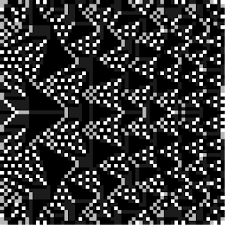
\includegraphics[width=0.43\textwidth]{abelian_sandpile.png}
    \caption{Cascading Abelian sandpile}
  \end{center}
\end{wrapfigure}

In the corner of the office, we see two piles of crumpled up balls of white papers on the ground, presumably containing the failed and abandoned ideas of Dr Prigogine. We can see that the piles are somewhat stable, so using our goggles we'd like to see how they respond to small fluctuations. We step back and look at the whole of one of the piles and slowly increase the complexity parameter until we see that the pile reaches a critical point where it loses all of its stability and collapses onto the floor. Next, we turn our sights to the second pile and move close enough to it so that we're focusing on a single ball of crumpled paper amongst the pile. Again, we introduce small fluctuations in the paper which pushes around other nearby crumpled papers. Not long after these small interactions, we see the same results as before, the pile as a whole loses its stability and crashes to the floor.

Earlier, we saw how predictions about future local states are often fallible because of their dependence on the interactions of the system as a whole. We're now seeing an alternative perspective of this fact: the small interactions of parts of a system can cause large changes and disruptions to the system as whole. These same findings were put forward by a group of three physicists in what's known as a \emph{Bak–Tang–Wiesenfeld model}\cite{btw}, metaphorically explained as a sandpile with new grains of sand being randomly added until the slope exceeds a given threshold which will then cause an avalanche. Just as our experiment had shown, their model demonstrated how the emergence of complexity from simple local interactions could explain spontaneous natural complexity rather than something only possible in artificial situations where control parameters of the entire system are tuned to precise critical values. The general behaviour was named \emph{self-organized critically} and contributed to the theory of self-organization, which refers to any process where some form of overall order or pattern arises from local interactions between the parts of an initially chaotic system. A classic example of self-organization is the swarm behaviour displayed in a large flock of birds.

\section{Dissapative Structures Outside the Office}
Standing in his office, we're immediately reminded of the work of Illya Prigogine. In the 1960s, Prigogine conducted research in dynamical systems, mainly in the physical science of thermodynamics. Thermodynamics involves heat and its transformation into other forms of energy using statistical descriptions of atomic and molecular movements. Prigogine became interested in an unpopular area of irreversible thermodynamics, which analyses processes where it is impossible to restore an environment back to its initial conditions after their occurrence, causing entropy and disorder. All sufficiently complex natural processes are considered irreversible, usually as a result of \emph{dissipation} or loss of energy which can occur when heat is transferred through thermal resistance or during some other atomic or molecular transformation.

His Nobel prize-winning theory had its origins in the realization that long before a state of balance is reached, irreversible processes could drive systems which were in thermal chaos to orderly and stable states\cite{ds}. This change could occur by artificially amplified fluctuations, similar to the effect of the goggles in our own experiments. Prigogine called these fluctuations \emph{dissipative structures} to emphasize the constructive role of these irreversible processes. Dissipation, which was previously considered a nuisance because of its creation of disorder was now causing self-organization, which we've learned creates a form of overall order in a chaotic system. Prigogine posited that this theory captured the key to understanding the origin of order and creativity we see in nature. The societal implications of the underlying philosophy of his experiments are expressed in his work Order out of Chaos\cite{oooc}
\begin{displayquote}
The threat lies in the realization that in our universe the security of stable, permanent rules are gone forever. We are living in a dangerous and uncertain world that inspires no blind confidence. Our hope arises from the knowledge that even small fluctuations may grow and change the overall structure. As a result, individual activity is not doomed to insignificance
\end{displayquote}

We've learned a great deal from the experiments we've performed in the confines of Illya Prigogine's office, and now we feel ready to run an experiment outside in the real world. As we leave the office, we look out into nature and society through Prigogine's goggles and see a vast array of chaotic systems. Some of them destructive, others unsustainable, and yet others in a perfect balance. Again, we stop for a moment to ask ourselves: with our newfound knowledge, what do we want to get out of our next experiment?


\begin{thebibliography}{4}

\bibitem{eoc}
Ranjit Kumar Upadhyay (2009). "Dynamics of an ecological model living on the edge of chaos". Applied Mathematics and Computation.

\bibitem{btw}
Bak, P.; Tang, C.; Wiesenfeld, K. (1987). "Self-organized criticality: an explanation of $1/f$ noise". Physical Review Letters.

\bibitem{ds}
Prigogine, I. (1978). Time, Structure, and Fluctuations. Science, 201(4358), 777-785. Retrieved March 22, 2020, from www.jstor.org/stable/1746122

\bibitem{oooc}
Prigogine, I., Stengers, I., (1984). Order out of chaos: Man's new dialogue with nature. Boulder, CO: New Science Library.

\end{thebibliography}
\end{document}
